\section{Experimental Evaluation}
\label{exp}
%%%%%%%%%%% 1st experiment %%%%%%%%%%%%
% {\color {red} We evaluate the ....using two sets pf experiments: ...The first exdpriment what why.... the second what why? } WHAT
% WHY?
% HOW? 
% experimenta setup
% -dateset
% - environment
% Results and discussion 

As each data feature has its own distributional properties in the training dataset, we assess the significant impact of data feature distributional shape including intrinsic properties like feature skewness, on the model performance (see Appendix~\ref{impact_app} for more details). We evaluate the proposed method by investigating the correlation of data opinion initialization as interpretable data opinions with the model performance. Since a DNN model with higher accuracy exhibits higher projected probability and lower uncertainty, we expect different input data opinion initialization impact the trustworthiness and total uncertainty of the DNN model. We assess our approach based on the presence of different statistical factors in initializing data opinions. We demonstrate that the belief, uncertainty, and trustworthiness, i.e., projected probability, will be improved in a DNN model based on its loss function optimization during training process. 

% The intrinsic distributional properties, for instance, the skewness or asymmetric distribution of input data, can impact the model performance since real-world data distributions are usually skewed. In skewed data, the tail area can act as an outlier, and outliers adversely influence the model performance. Thus, the skewed data should be transformed to be adequately close to a normal distribution. 

%%%%%%%%%%%%%%%%%%%%%%%%%%%%%%%%%%%%%%%
% In this research, the assessment goal is to use model performance (accuracy) and loss as measures to evaluate our approach such a way that we expect a DNN model with higher accuracy indicates lower uncertainty with respect to the various input data opinion initialization. We show that the belief and uncertainty will be improved in a DNN model based on its loss function optimization during training process. 

\vspace {.2cm}
\noindent
\textbf{Datasets.}
We have evaluated the proposed method on two real-world datasets: 1) SUSY dataset\footnote{\url{https://archive.ics.uci.edu/ml/datasets/SUSY}} with 5 million samples from particle physics community containing 18 features, two target labels, and no missing/misleading data values~\cite{susy}, 
2) KDD Cup 99 dataset\footnote{\url{https://archive.ics.uci.edu/ml/datasets/KDD+Cup+1999+Data}}, with 4 million samples from computer network logs used for intrusion detection task containing 41 features (including categorical features), three selected target labels, and no missing/misleading data values~\cite{kdd}.

\vspace{.2cm}
\noindent
\textbf{Evaluation Setup.}
We implemented the proposed data opinion propagation method in Python\footnote{The source code is available at: \url{https://github.com/[NAME REMOVED]/sl-uncertainty}}, and the assessments have been performed on a machine with Intel(R) Core(TM) i7-10750H 2.60GHz (6 cores) processor and 16GB RAM allocated to our computation. 

%Since both datasets are relatively balanced in the number of their target classes. 
To run our experiments, we ensured the datasets were almost balanced, and the data were encoded (categorical features) and normalized. We ran the experiments over 15\% of the entire data points for each dataset with 80\% training and 20\% testing sampling. We utilized a 4-layer neural network with 20-10 and 30-15 neurons in the hidden layers to train and test the model on Susy and KDDCUP99 datasets over 50 and 20 training epochs, respectively. In addition, we exploited the Cross-Entropy loss function and Adam optimizer with an initial learning rate of 0.001 to train our classifiers. {\color{blue}The learning rates used in this paper are the initial ones for the adaptive optimization process using the Adam optimizer. Note that this approach is a topology agnostic method based on the experiments in~\cite{hope}. Therefore, Although different DNN architectures may impact the total model accuracy and then model trustworthiness, this method is applicable by any arbitrary DNN architecture.}

\subsection{Results and Interpretations}
{\color{blue}
\noindent \textbf{A Preliminary Experiment.} As the first part of the evaluations, a preliminary experiment is performed to demonstrate how the distributional properties in input data can impact the model performance. We used Pima Indians Diabetes Dataset\footnote{\url{https://www.kaggle.com/datasets/uciml/pima-indians-diabetes-database}} originally from the National Institute of Diabetes and Digestive and Kidney Diseases. 

We apply a classification task using different traditional classifiers like K-nearest, Logistic Regression, Random Forest, AdaBoost, and a DNN classifier (\emph{MLPClassifier} with three layers optimized by Adam and with an initial learning rate of 0.01) on both original distributions (e.g., skewed) and transformed distributions (e.g., no longer skewed). 
%K-nearest, Logistic Regression, Random Forest, AdaBoost, and Bagging classifiers on the original and transformed data features. 
%For the DNN classifier, we used \emph{MLPClassifier} as a three-layer neural network model optimized by Adam and initial learning rate of 0.01. 
In Figure~\ref{skew_dist}, the distribution of the three most skewed features of the dataset named \emph{Insulin}, \emph{DiabetesPedigreeFunction}, and \emph{Age}, as well as the transformed features, are shown. Therefore, in Figure~\ref{skew_acc}, we can see the accuracy of different classifiers including the DNN model over the original and transformed distributions of the most skewed features that hold the highest skewness and kurtosis in this dataset.
\begin{figure}[t]  % H
\centering
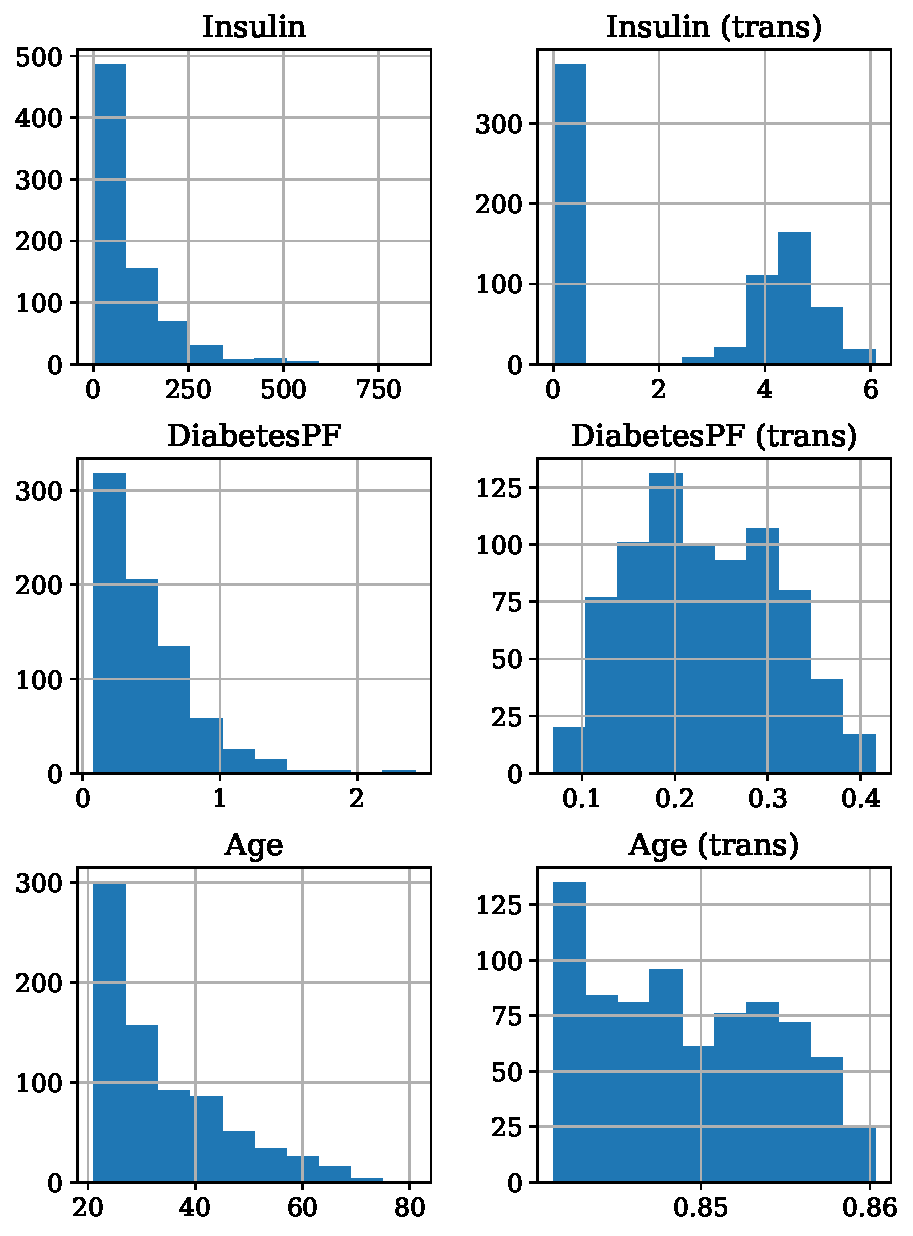
\includegraphics[width=0.4\textwidth]{figures/dist.pdf}
\vspace{-0.3cm}
\caption{The original and transformed distributions of the three most skewed features of the Pima Indians Diabetes Dataset}
\label{skew_dist}
\end{figure}
\begin{figure}[t]  % H
\centering
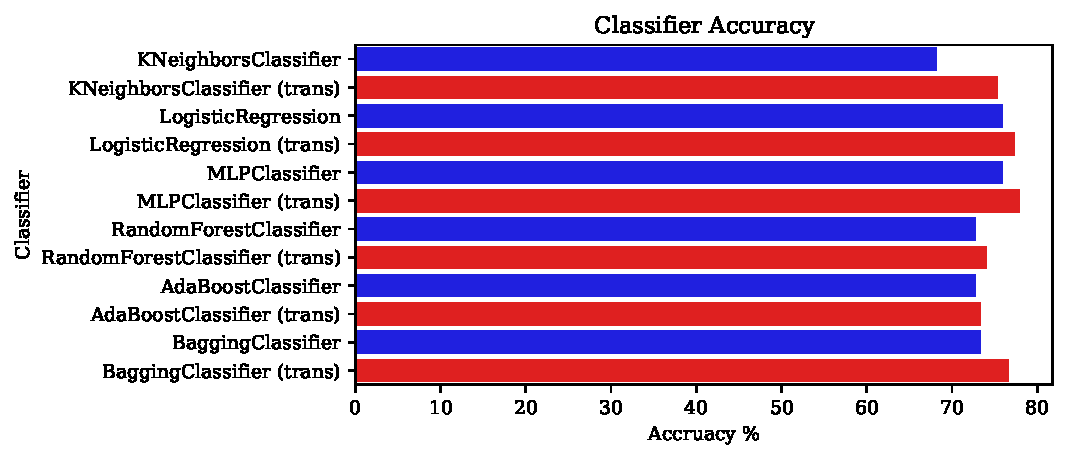
\includegraphics[width=0.5\textwidth]{figures/classifiers.pdf}
\vspace{-0.7cm}
\caption{The model accuracy of different classifiers based on the original (green bars) and transformed (red bars) distributions of the three most skewed features of the Pima Indians Diabetes Dataset}
\label{skew_acc}
\end{figure}

\begin{figure*}[!ht]  % H
	\centering % width=\textwidth
	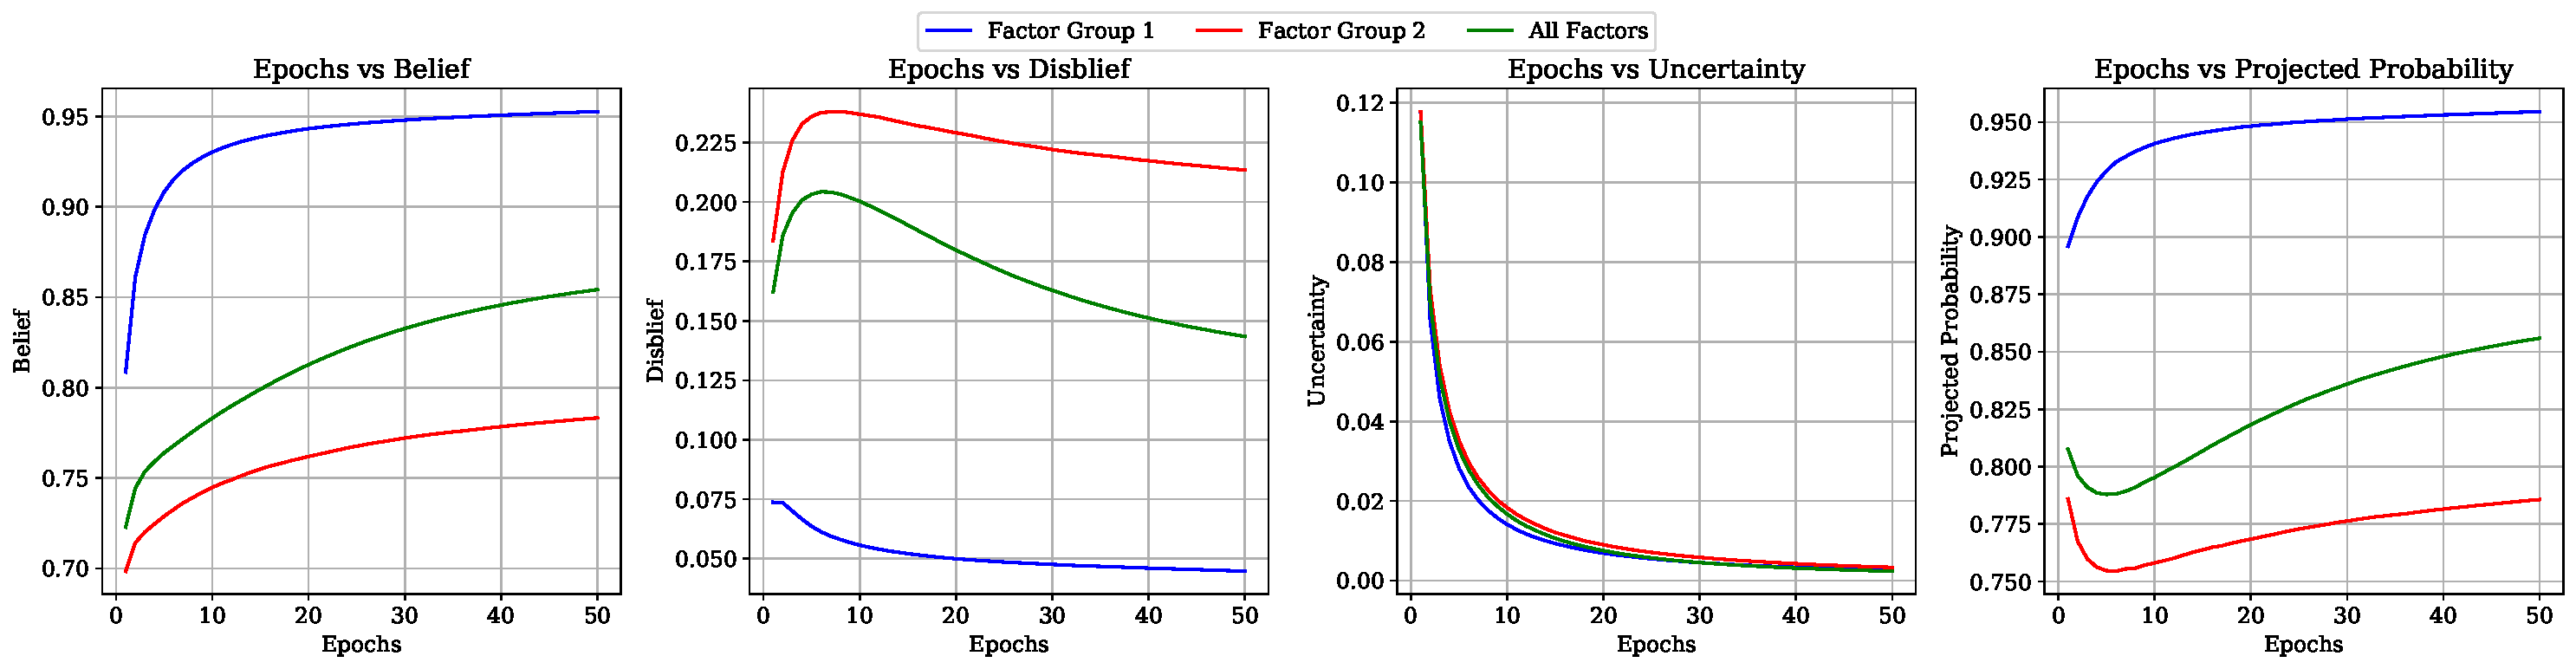
\includegraphics[width=0.8\textwidth]{figures/Results_Op_susy.pdf}
	\vspace{-0.3cm}
	\caption{The average improvement process of opinion determinants during 50 training epochs over 5 different runs based on different factors in numerical features for SUSY dataset}
\label{susy_op}
\end{figure*}
\begin{figure*}[!ht]
	\centering % width=\textwidth
	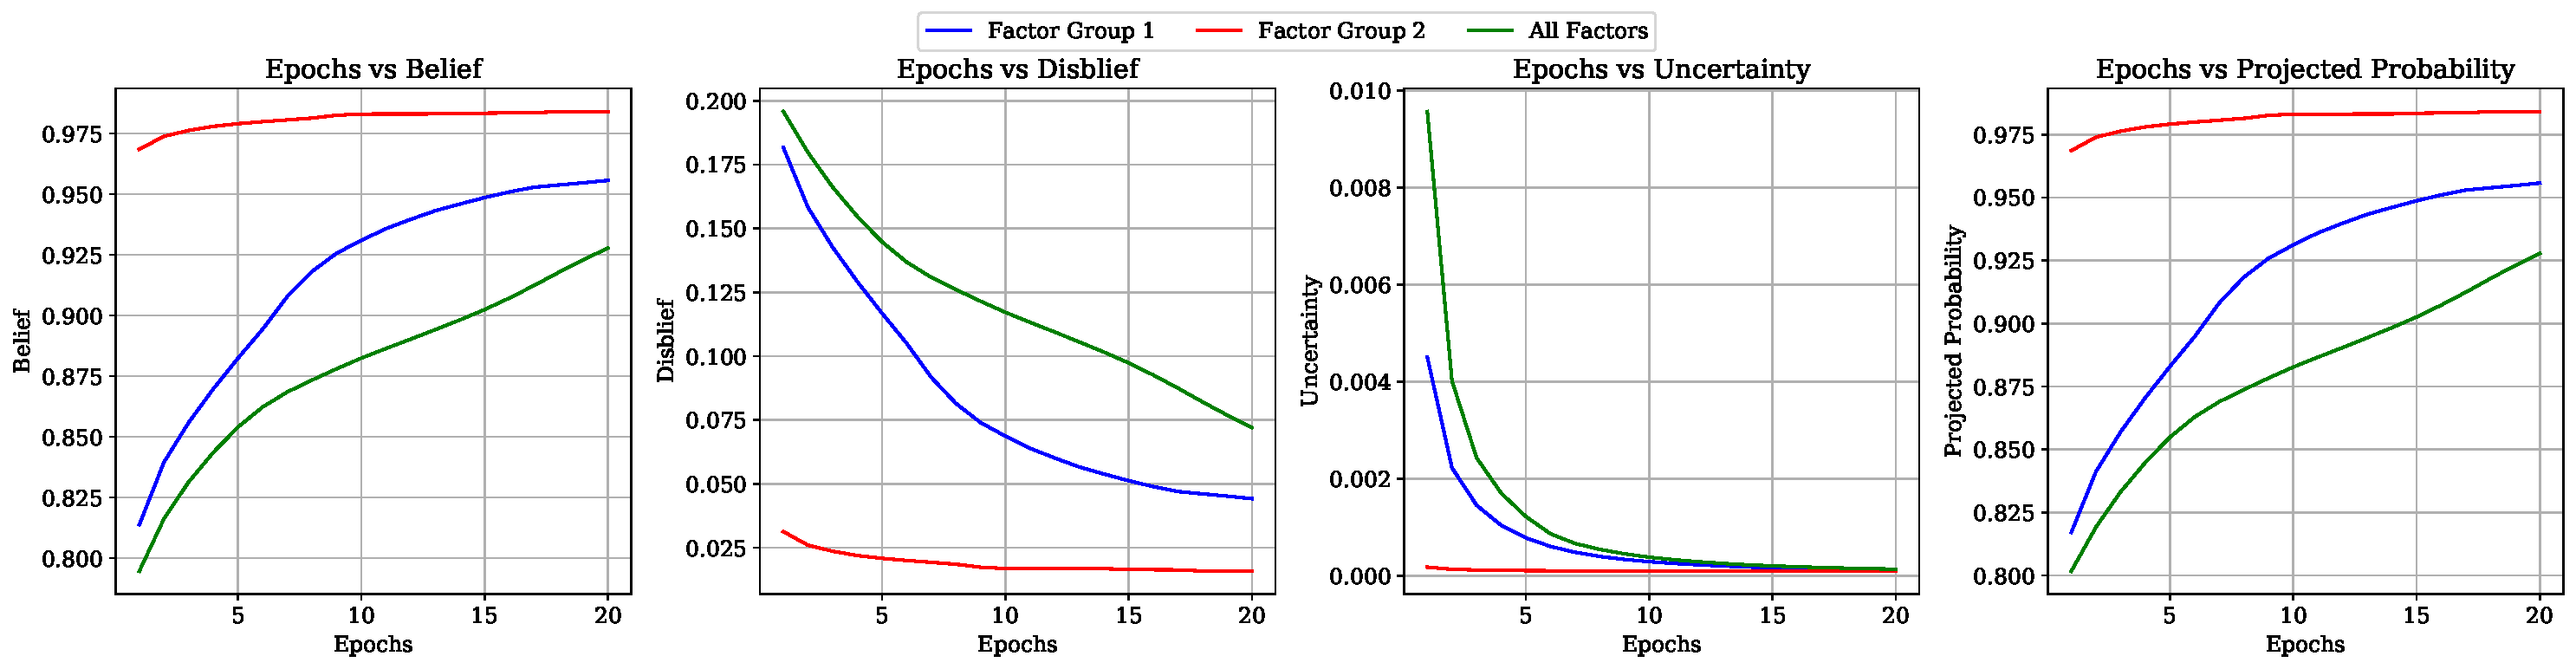
\includegraphics[width=0.8\textwidth]{figures/Results_Op_kdd.pdf}
	\vspace{-0.3cm}
	\caption{The average improvement process of opinion determinants during 20 training epochs over 5 different runs based on different factors in numerical features for KDD CUP 99 dataset}
\label{kdd_op}
\end{figure*}

The results show that the transformed feature distribution mitigates the skewness and kurtosis as two distributional properties of training data. We can see the accuracy improvement of all classifiers in the presence of transformed features. Therefore, the skewed training data features that also have higher kurtosis, can negatively impact the DNN performance. This result also indicates the necessity of considering statistical and distributional properties of input data in initializing data opinions before propagation through the DNN network.
}

\noindent \textbf{Main Experiments.} Since the datasets used to train DNN models can be considerably different in terms of their statistical properties, we used the equally-weighted average of two distinct groups of statistical factors for each data opinion determinant in each dataset. We run the experiment for two groups of statistical factors mentioned in Section~\ref{op_init_sec}. 
% Cronbach's Alpha, Data Quality Score (DQS), and Eigenvalue ratio (explained variance) as the first group and Skewness, Kurtosis, and the Distributional Variance as the second group. 
We first run the experiment for each group of factors separately and then together. In Figures~\ref{susy_op} and~\ref{kdd_op}, there are two lines, blue and red, indicating the change in model opinion determinants as well as the model projected probability considering the first and second group of data opinion initialization factors, respectively. The green line also indicates the change in model opinion determinants and its projected probability considering both sets of factors simultaneously, by the equally-weighted average. During training epochs, in Figures~\ref{susy_op} and~\ref{kdd_op}, we can see the increasing change in model belief as well as the decreasing change in model uncertainty for both datasets considering different factors separately and together.{\color{blue} Therefore, model belief and uncertainty are relatively improved during training epochs in a way that belief is increased while uncertainty is decreased. Finally, we can observe that during the training process, the model trustworthiness or projected probability is increased when there is no significant increasing change in disbelief. 

As the results show, arbitrary selection of statistical factors to initialize the input data opinions may impact the total model trustworthiness. Therefore, this approach is flexible enough in selecting different statistical factors based on the application, data type, research domain, and the objective of the classification task. However, using the weighted average of the most correlated factors in initializing each determinant of interpretable data opinions will lead to a more realistic view of the model trustworthiness because of considering more aspects of data distribution in a batch of training data. Note that as mentioned before, we use equally-weighted average of distinct factors in initialization process. Therefore, based on the application and task domain, different weights can be assigned to different factors for averaging to tune the importance and priority of some specific statistical factors.}

{\color{blue}
Furthermore, Figures~\ref{susy_loss} and~\ref{kdd_loss} illustrate that the training processes over both SUSY and KDD Cup 99 datasets are performed effectively as decreasing loss and increasing accuracy during the training process shown in these figures is a sign of a successful learning process.}
%(see Appendix~\ref{train_app})
A successful training process leads to an increase in model belief and projected probability as a measure of trustworthiness for both datasets while our model uncertainty is decreasing significantly. Thus, the projected probability is positively correlated with the model performance, and we can trust the DNN model much more than before after a successful training process. In comparison with the other trained models in the case of similar accuracy, we can decide to select the model with a higher projected probability at first, and in case of no significant discrepancy, the model with higher belief, lower disbelief, and lower uncertainty will be selected. In addition, we see insignificant change in the amount of disbelief (approximately less than 0.1) during training, which is convincing since our input data that fed to the DNN were of high quality without data type mismatch or any missing or misleading data records. 

{\color{blue} The low-quality input data may have missing and misleading data points or data type mismatch that give rise to input data with higher disbelief and lower trustworthiness. In Figures~\ref{susy_miss} and~\ref{kdd_miss}, we demonstrate the behavior of the proposed method in the presence of input data with lower quality. In this regard, we experiment the proposed method on both datasets with different ratios of missing/misleading data points. The results show that the lower quality input data with lower trustworthiness have higher model disbelief along with an increase in model disbelief during training rather than input data with higher quality. Therefore, we can observe that the more missing/misleading data ratios are in the datasets, the more model disbelief and the less model belief and trustworthiness (projected probability) we achieve during training epochs. We can also observe that low-quality data with lower trustworthiness may decrease the model belief and eventually, decrease the model trustworthiness during the training phase.         
}

We report the average performance results as well as initial and ultimate model opinions during five distinct runs for each dataset in Table~\ref{result}. In this table, the model opinion determinants for training and testing phases over each dataset are updated and improved based on the loss function and accuracy achieved during a total number of training epochs. Note that the total belief and projected probability or trustworthiness of the model have been increased compared to the first epoch of training while the uncertainty has been relatively decreased. This result confirms the impact of successful training and loss optimization on the quantification and propagation of the total opinion's determinants. 
% As the loss function is being minimized during training epochs, the accuracy of the entire network is increasing. Therefore, the model accuracy in training time is correlated to the belief and uncertainty of the model opinion. 
% Since the opinion determinants have an additivity requirement, change in one determinant coincides with changes in other determinants. 
% We can also see the improvement in the trustworthiness or projected probability of the model while training is performed. Note the difference between the projected probability in total opinion (after training) compared to the first epoch of training such that the total projected probability of the model has been increased compared to the starting point of training. Note that we could achieve better performance by hyperparameter tuning and/or increasing the number of training epochs. However, this improvement was irrelevant to the objectives of the experiment.  

\begin{table*}[!ht]
% \hskip -1.3cm
\centering
\caption{The average performance and opinion results for training and testing phases during 5 different runs over each dataset}
\vspace{-0.1cm}
\begin{tabular}{c c cccc cccc}
    \toprule
\multirow{2}{*}{\textbf{Dataset}} 
        & \multicolumn{1}{c}{\textbf{Performance}} & \multicolumn{4}{c}{\textbf{1st Training Epoch Opinion}} &
        \multicolumn{4}{c}{\textbf{Total Opinion}} \\
    \cmidrule(lr){2-2} \cmidrule(lr){3-6} \cmidrule(lr){7-10}
        & Total Accuracy & Belief & Disbelief & Uncertainty & Proj. Prob. & Belief  & Disbelief & Uncertainty & Proj. Prob. \\
    \midrule
SUSY: \textit{Training} 
        & 72.863\%  & 0.6420 & 0.0160 & 0.3420 & 0.8130 & 0.8470 & 0.0080 & 0.1440 & 0.9640      \\
    \addlinespace
SUSY: \textit{Testing}
        & 69.785\%   & - & - & - & - &  0.8495 & 0.0089 & 0.1417 & 0.9203        \\
    \addlinespace
KDDCup99: \textit{Training}
        & 99.065\%  & 0.9280 & 0.0050 & 0.0670 & 0.9610 & 0.9978 & 0.0002 & 0.0021 & 0.9981 \\
    \addlinespace
KDDCup99: \textit{Testing}
        & 97.846\%   &  -   &  -  &  -  & - &  0.9969 & 0.0002 & 0.0029 & 0.9970    \\
    % \addlinespace

% \multirow{4}{*}{KDD Cup 99}
%         & item 1    & item 2    & then 3    & item 4    & item 5    & item 6            \\
%         & item 1    & item 2    & then 3    & item 4    & item 5    & item 6            \\
%         & item 1    & item 2    & then 3    & item 4    & item 5    & item 6            \\
%         & item 1    & item 2    & then 3    & item 4    & item 5    & item 6            \\
    \bottomrule
\end{tabular}
%\vspace{-0.5cm}
\label{result}
\end{table*}

% In addition, any suitable value for each hyperparameter in our model like the number of required training epochs for convergence, the initial amount of learning rate, and the optimization approach can be leveraged to achieve the best possible accuracy.

In conclusion, our evaluation demonstrates that the opinion quantification process is adequately flexible when statistical properties of the input data are incorporated into the process. Note that the selection of these statistical factors can be different from one model to another based on the characteristics of the application domain. For example, in the medical domain, the reliability of input data could be a major factor in the opinion generation while in another domain, the skewness or kurtosis of data can have higher priority to be considered.

%Another advantage of incorporating statestical poroperties of input data in opinion propagation is its contribution to the interperqatbility and explainability of the  is the 


%charactristicsstatistical properties of the input dataset. These independent factors for data opinion initialization should be explainable and interpretable based on the nature of feature distributions, the task objective, and the application domain. We can also apply different weights for different factors in the proposed approach to tune the impact of each factor in initializing data opinion determinants. 

%the proposed data opinion propagation approach is adequately flexible for different DNN architectures.

%since based on the nature of input data and its features, any appropriate architecture of neural network can be utilized to train the model and achieve the best possible performance. 

%initialization approach for data feature opinions is constructed based on statistical properties of input data, also comprehensively flexible. Everyone can exploit and add more different and independent statistical factors, combined by weighted average, to initialize the data opinion determinants, even for the categorical features' opinions as well. 

\begin{figure}[ht]  % H
\centering
% \vspace{-10cm}
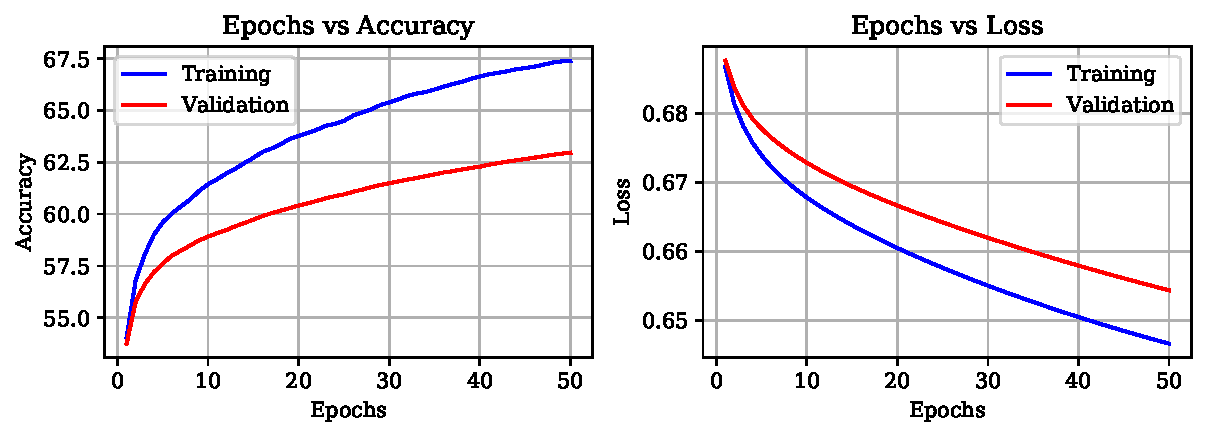
\includegraphics[width=0.5\textwidth]{figures/Results_susy.pdf}
%\vspace{-0.3cm}
\caption{The accuracy and loss values for training and validation phases during 50 training epochs over SUSY dataset}
\label{susy_loss}
\end{figure}

\begin{figure}[ht] % H
\centering
% \vspace{-22cm}
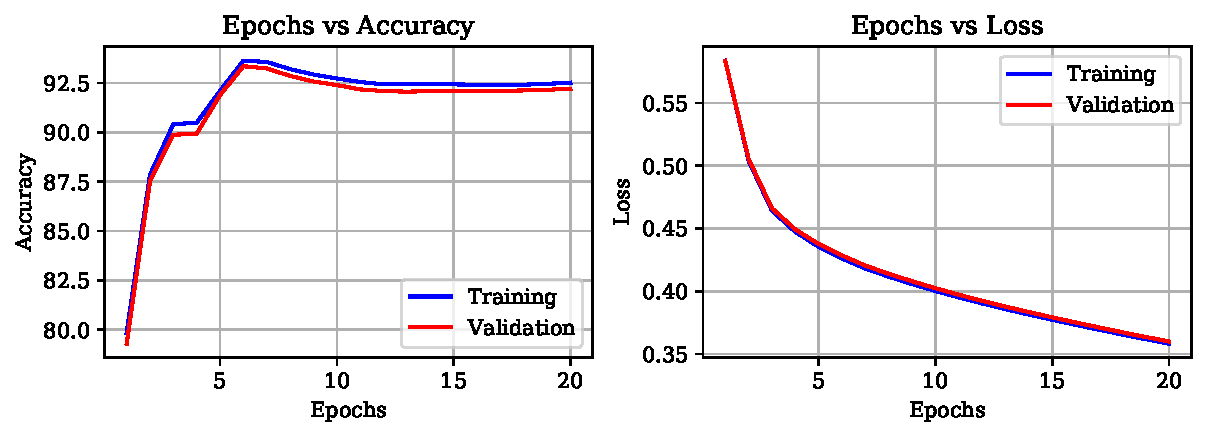
\includegraphics[width=0.5\textwidth]{figures/Results_kdd.pdf}
%\vspace{-0.3cm}
\caption{The accuracy and loss values for training and validation phases during 20 training epochs over KDD CUP 99 dataset}
\label{kdd_loss}
\end{figure}

\begin{figure*}[!ht]  % H
	\centering % width=\textwidth
	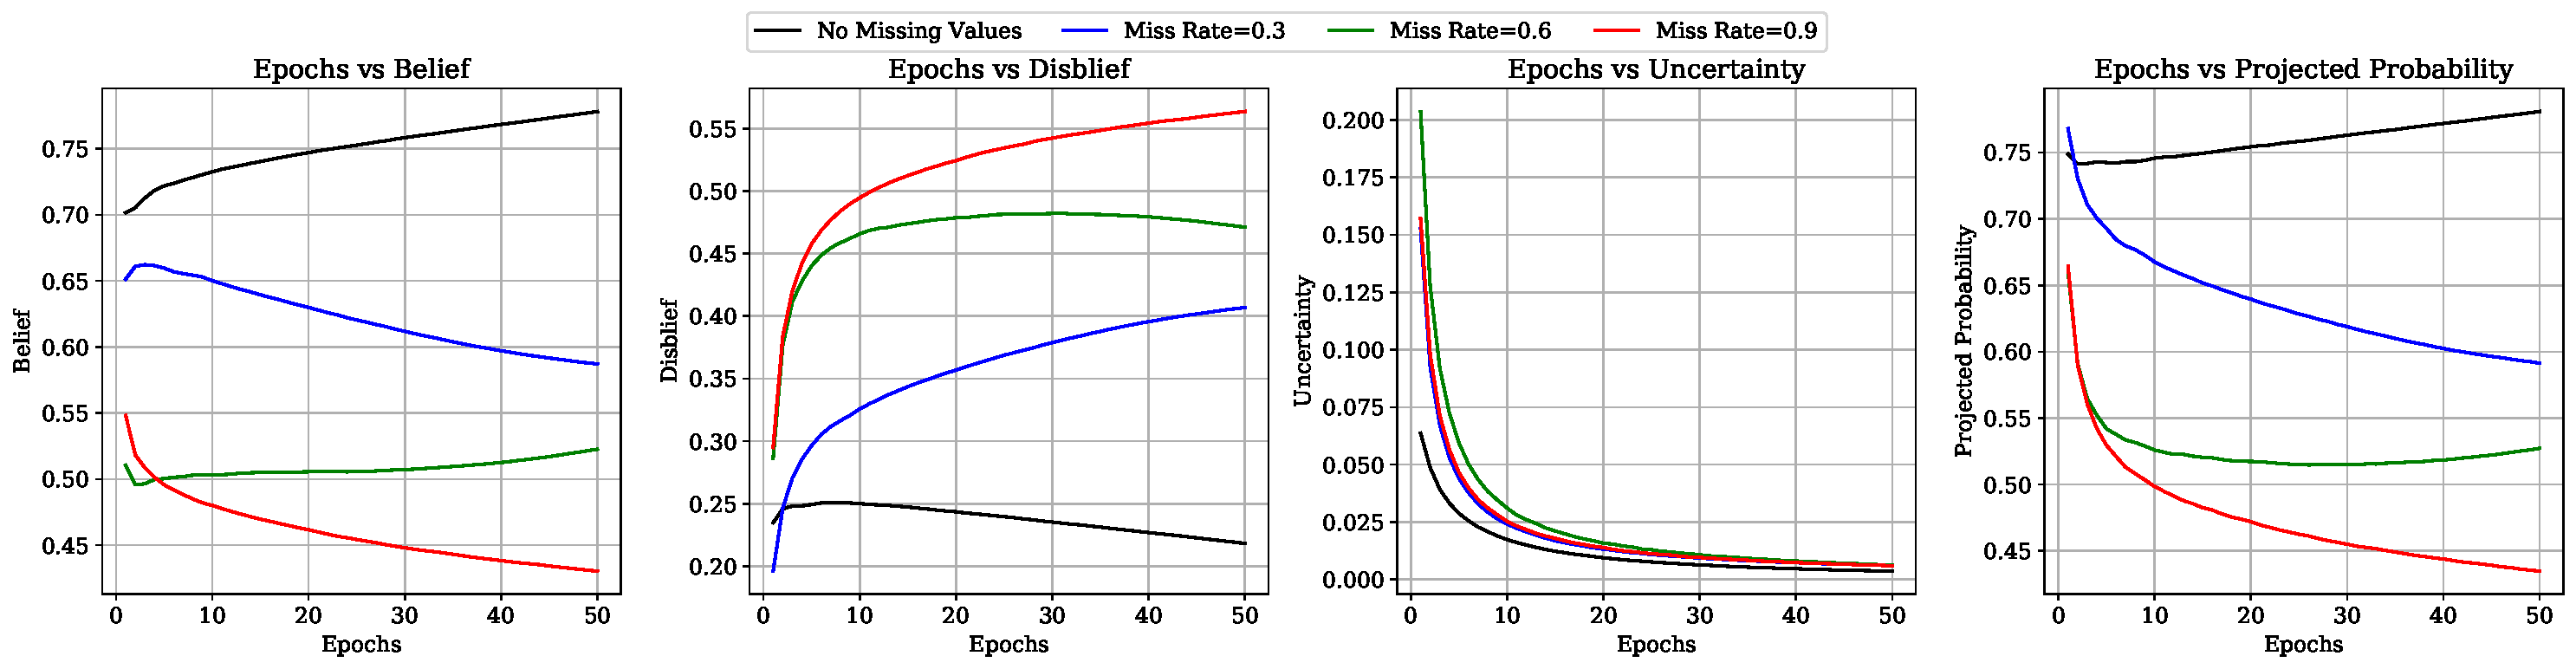
\includegraphics[width=0.8\textwidth]{figures/Results_susy_miss.pdf}
	\vspace{-0.3cm}
	\caption{The improvement process of opinion determinants during 50 training epochs over training data with different level of trustworthiness based on different miss rate for SUSY dataset}
\label{susy_miss}
\end{figure*}

\begin{figure*}[!ht]
	\centering % width=\textwidth
	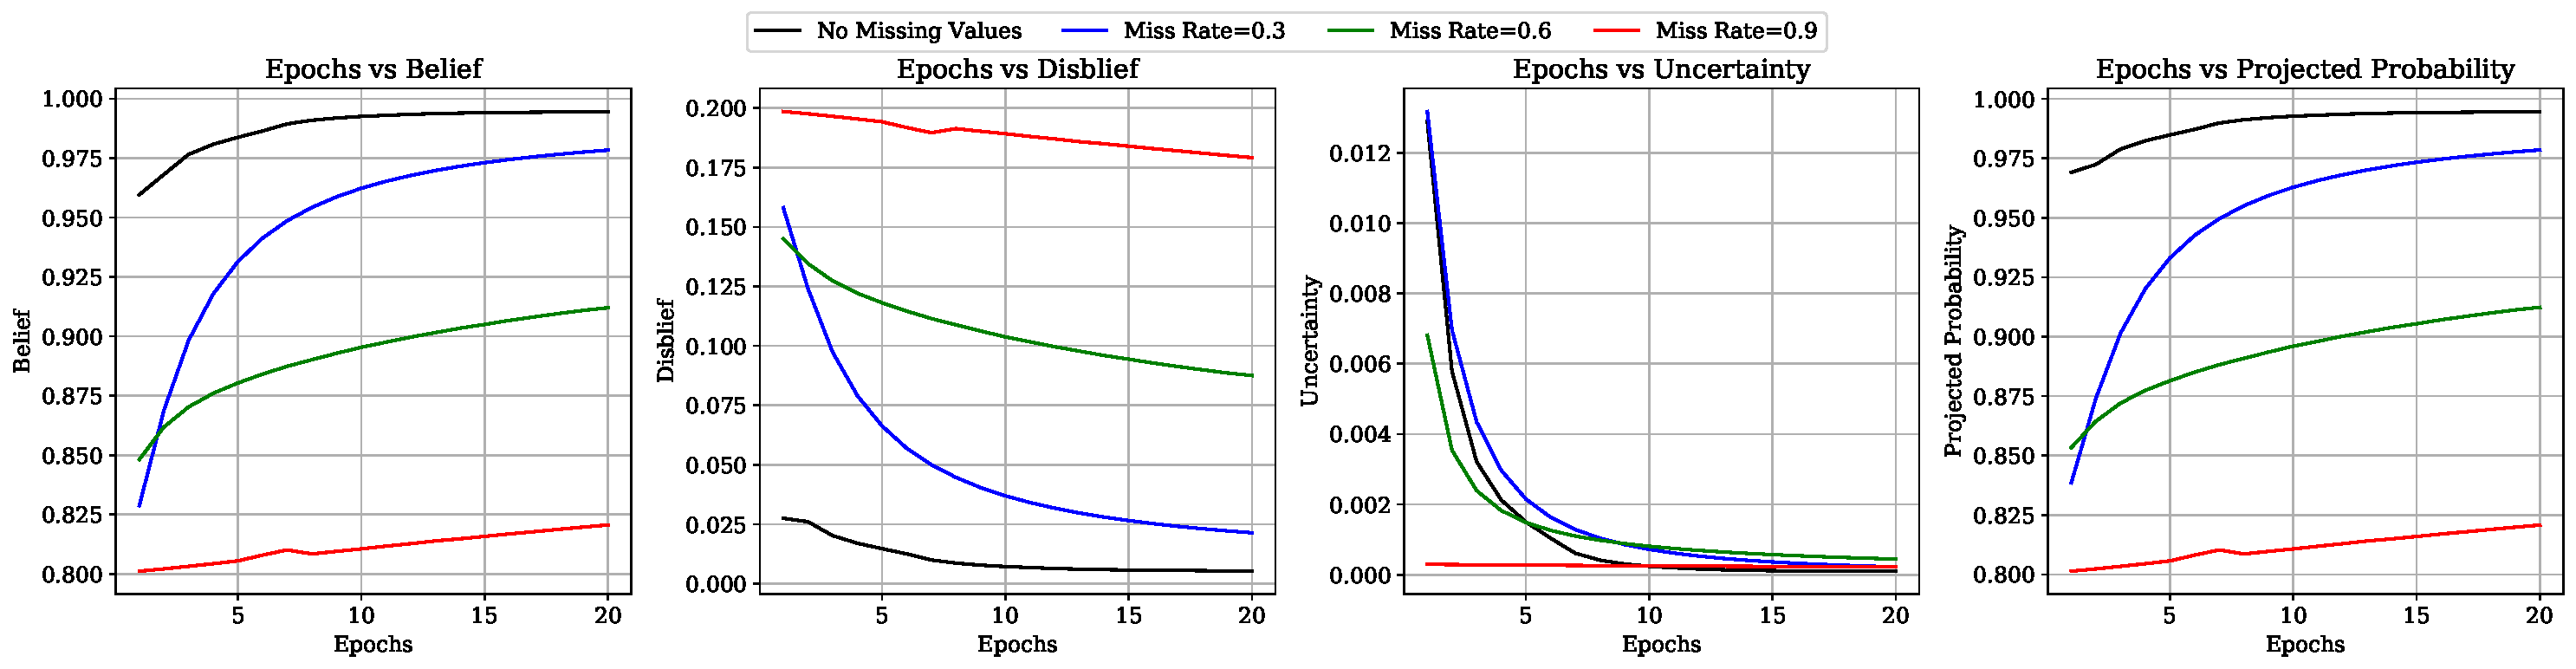
\includegraphics[width=0.8\textwidth]{figures/Results_kdd_miss.pdf}
	\vspace{-0.3cm}
	\caption{The improvement process of opinion determinants during 20 training epochs over training data with different level of trustworthiness based on different miss rate for KDD CUP 99 dataset}
\label{kdd_miss}
\end{figure*}









% Confusion matrices in the Figure~\ref{susy_cm} and~\ref{kdd_cm} demonstrate that the trained model could achieve good results and acceptable accuracy over unseen data (test data).

% \begin{figure}[H]
% 	\centering
% 	\includegraphics[scale=0.5]{figures/susy_cm.PNG}
% 	\caption{A Confusion matrix for testing over SUSY dataset}
% 	\label{susy_cm}
% \end{figure}
% \begin{figure}[H]
% 	\centering
% 	\includegraphics[scale=0.5]{figures/kdd_cm.PNG}
% 	\caption{A Confusion matrix for testing over KDD Cup 99 dataset}
% 	\label{kdd_cm}
% \end{figure}


%%%%%%%%%%%%%%%%%%%%%%%%%%%%%%%%%%%%%%%%%%%%%%%%%%%%%%%%%%%%%%%

% \usepackage{booktabs, multirow}


% \begin{table}
% \centering
% \begin{tabular}{c ccc ccc}
%     \toprule
% \multirow{2}{*}{two rows} 
%         & \multicolumn{3}{c}{3-columns cell} & \multicolumn{3}{c}{3-columns cell}   \\
%     \cmidrule(lr){2-4} \cmidrule(lr){5-7}
%         & column 1  & column 2  & column 3  & column 4  & column 5  & column 6          \\
%     \midrule
% \multirow{4}{*}{Social Network}  
%         & item 1    & item 2    & then 3    & item 4    & item 5    & item 6            \\
%         & item 1    & item 2    & then 3    & item 4    & item 5    & item 6            \\
%         & item 1    & item 2    & then 3    & item 4    & item 5    & item 6            \\
%         & item 1    & item 2    & then 3    & item 4    & item 5    & item 6            \\
%     \addlinespace
% \multirow{4}{*}{Citation Dataset}
%         & item 1    & item 2    & then 3    & item 4    & item 5    & item 6            \\
%         & item 1    & item 2    & then 3    & item 4    & item 5    & item 6            \\
%         & item 1    & item 2    & then 3    & item 4    & item 5    & item 6            \\
%         & item 1    & item 2    & then 3    & item 4    & item 5    & item 6            \\
% \bottomrule
% \end{tabular}
% \caption{Example of professional table design}
%     \end{table}


% \begin{table}[t]
% \begin{tabular*}{\columnwidth}{@{\extracolsep{\fill}}%
%     l T{4}T{2}T{2}T{4}}
% \toprule
% Year & {Nones}& {Option 1} & {Option 2} & {Total} \\
% \midrule
%   2001& 126   & 16    & 2     & 144 \\
%   2002& 114   & 9     & 4     & 127 \\
%   2003& 115   & 7     & 1     & 123 \\
%   2004& 114   & 6     & 4     & 124 \\
%   2005& 104   & 5     & 8     & 117 \\
%   2006& 96    & 3     & 6     & 105 \\
%   2007& 93    & 2     & 4     & 99 \\
%   2008& 93    & 2     & 2     & 97 \\
%   2009& 85    & 2     & 11    & 98 \\
%   2010& 83    & 0     & 7     & 90 \\
%   2011& 74    & 0     & 12    & 86 \\
%   \midrule
%   Total & 1097 & 52   & 61    & 1210 \\
% \bottomrule
% \end{tabular*}
% \end{table}



% \begin{table*}
% %
% \tablestyle[sansbold]
% %
% \begin{tabular}{*{2}{p{0.45\textwidth}}}
% \theadstart
%     \thead header &
%     \thead header \\
% \tbody
%  %
%  content  & content \\
%  content  & content \\
%  content  & content \\
%  %
%  \tsubheadstart
%  \tsubhead subhead &
%  \tsubhead subhead \\
%  %
%  content  & content \\
%  content  & content \\
%  \tend
% \end{tabular}
% \vspace{2mm}
% \caption{sansbold style}
% \label{tab:style:sansbold}
% \end{table*} 